163. Если провести высоту (и медиану) $BH,$ то $HC=AC:2=7,\ BH=\sqrt{625-49}=24.$ Тогда $S_{\Delta ABC}=\cfrac{1}{2}\cdot24\cdot14=168.$\\
а) Найдём площадь треугольника через проведённую из точки $C$ высоту $h:\ S=\cfrac{1}{2}h\cdot25=168,\ h=\cfrac{336}{25}.$\\
б) Найдём площадь треугольника через радиус вписанной окружности: $p=\cfrac{25+25+14}{2}=32,\ S=pr=32r=168,\ r=\cfrac{21}{4}.$\\
в) Найдём площадь треугольника через радиус описанной окружности: $S=\cfrac{abc}{4R}=\cfrac{25\cdot25\cdot14}{4R}=168,\ R=\cfrac{625}{48}.$
ewpage
oindent
г) \begin{figure}[ht!]
\center{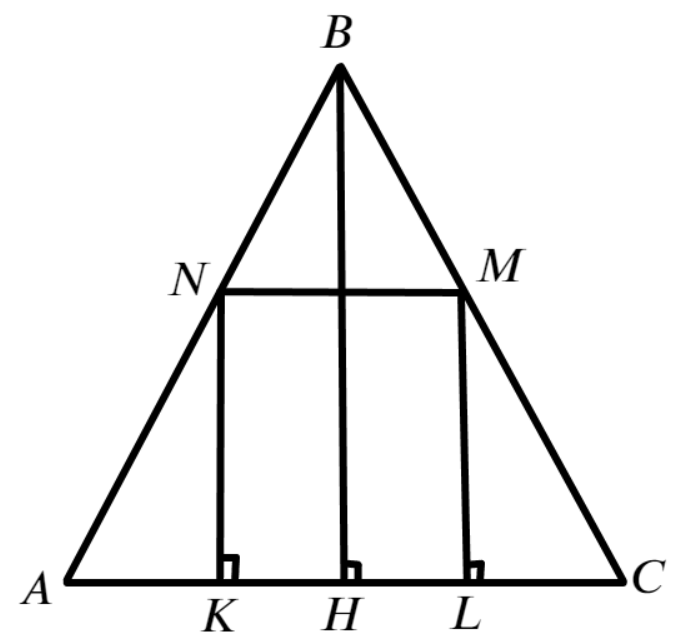
\includegraphics[scale=0.35]{g9-110.png}}
\end{figure}\\
Найдём $ctg(\angle A)=ctg(\angle C)=\cfrac{7}{24}.$ Тогда $AK=LC=LM\ ctg(\angle C)=\cfrac{7}{24}LM$ и $AC=2LC+KL=2\cdot\cfrac{7}{24}LM+\cfrac{1}{2}LM=\cfrac{13}{12}LM=14.$ Поэтому $KL=\cfrac{1}{2}LM=\cfrac{1}{2}\cdot\cfrac{168}{13}=\cfrac{84}{13}.$\\
